\documentclass[10pt,a4paper,twocolumn]{article}

\usepackage[T1]{fontenc}
\usepackage[utf8]{inputenc}

\usepackage[english]{babel}
\usepackage{natbib}
\usepackage{url}

\usepackage{graphicx, grffile}
\graphicspath{{../assets/}}

\usepackage{booktabs}

\title{Personal Reflections: Some thoughts on writing}
\author{Nazarov Ivan}

\begin{document}
\maketitle

I, personally, find the following guidelines and methods useful and productive for
writing text and pouring thoughts onto digital medium. They may be naive or silly, but
it think it is worth documenting them here. By the way this text itself may not follow
them by the letter, but hopefully does not gravely violate them.

Below is a brief recollection of what urged me to compose this scribble in early
Autumn of 2019:
\begin{quote}
  I used to follow them, but then lost my way due to stress and personal issues and
  forgot what it feels to actually `Feel` these principles. Luckily, such us the human
  nature, that one Wednesday evening, feeling particularly down from the paper that
  dragged on and on, I decided to force myself into not putting fragments, but complete
  thoughts into the text. I began a new document and pushed myself into getting a hold
  of my scattered ideas about composing text, they once again dawned onto me. I seem
  to have rebounded.
\end{quote}

Anyway, below are the guidelines, that strive for one goal: writing better quality
narrative in my academic/personal texts (not that many have been written so far, though).

\section{Avoid sentence/thought fragments} % (fold)
\label{sec:avoid_sentence_thought_fragments}

As soon as possible and not later, but always coalesce fragments into complete sentences
and/or coherent text fragments.

The train of thought is orders of magnitude faster than typing. Thus it is permitted
to write sentences/text out of order, skipping ahead to compose the ending or key phrases,
and backtracking afterwards to fill in the gaps. Place the pieces where ever they seem
to be relevant or belong in the tentative plan of the text.

Try to formulate what you want to write (at least crudely and partially) before actually
writing -- some planning and thought does ignite the mind and put you in the "flow".
It is not forbidden to type and design a sentence in Russian (native language), before
actually translating it to English.

% section avoid_sentence_thought_fragments (end)

\section{Fractal text structuring} % (fold)
\label{sec:fractal_text_structuring}

The overall narrative follows the classic structure: from general to specific. We introduce
something, develop it, draw conclusions, and move on either by getting more specific, or
shifting focus onto the connected topic or related concept. Focus on a single idea within
a paragraph, section, plot, or table.

Paragraph contains one complete piece of thought and its structure is the same: intro-%
main-outro, -- with cohesive devices interspersed here and there to string them together.
Paragraphs themselves exist within this narration flow: some paragraphs introduce, other
relay ideas concepts and the rest summarize or draw conclusion from the narrative in the
former.

% section fractal_text_structuring (end)

\section{The text is malleable material} % (fold)
\label{sec:the_text_is_malleable_material}

Writing text can benefit from programming styles and techniques. Adopt modular hierarchical
treatment of sentences, paragraphs, and sections. Top-down writing style works wonders:
begin with coarse plan, then progressively refine its element and ultimately being
coalescing the letters into words into phrases, into sentences, into paragraphs and
sections.

Always try to come up with synonyms when writing sentences -- this increases variety,
and broadens the perspective.

% section the_text_is_malleable_material (end)

\section{Iterative process} % (fold)
\label{sec:iterative_process}

Writing text is an iterative process of constant addition, removal, refinement and
revision. Just like research: submit for feedback, update, then rinse and repeat.

\begin{figure}
  \centering
  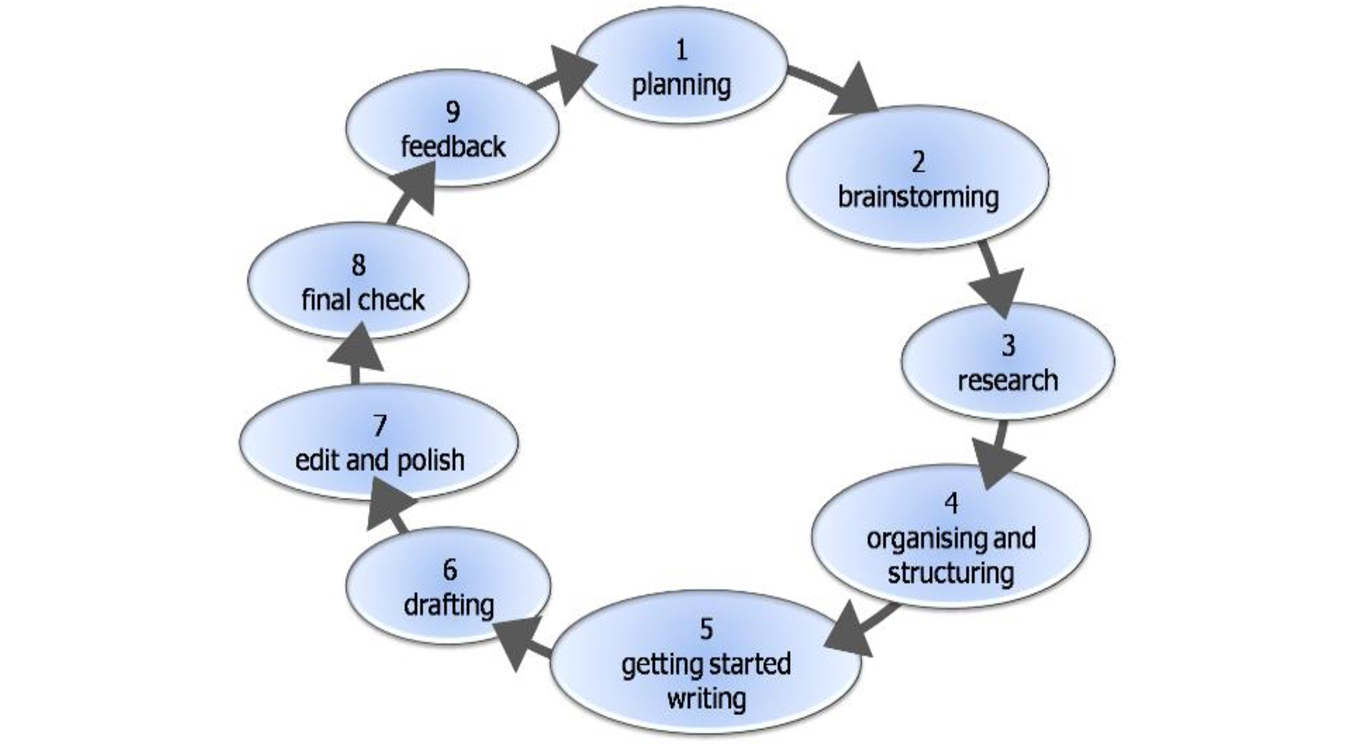
\includegraphics[width=\columnwidth]{assets/iterative_process.pdf}
  \caption{
    The cycle process of writing.
  }
\end{figure}

% section iterative_process (end)

\section{General narrative guidelines} % (fold)
\label{sec:general_narrative_guidelines}

The following rules are mostly listed as imperatives.

Don't include things (text, sentence, ideas) that are not your point. Do not add a formula
just for the sake of a formula. The narrative must flow: introduce concepts before using
them, refer to them as necessary, or even reproduce their condensed versions when needed.
Connect and develop ideas within text: what is the focus now builds upon what came before.
Try to keep related things close to each other -- that way it requires much less cognitive
load to understand the main idea of the paragraph, section or text.

% section general_narrative_guidelines (end)

\section{Writing in research} % (fold)
\label{sec:writing_in_research}

Writing must be an integral part of research activity, not a step done after the experiments.
In science you start with a hypothesis, test it then toss it out -- all of this reflected
in text. Text is dispensable: each writing activity is useful, but do not cling to text,
code or any other literary expression.

Having many drafts is normal and encouraged: each draft must be checked for assumptions,
terminology, logical correctness.

% section writing_in_research (end)

\end{document}
